\chapter{Filter Construction and Methodology}
\label{cha:method}

In this chapter, a method is proposed to solve the heading estimation problem.
The main idea is to compute how the front (or the back) of the target has moved between two consecutive frames, \ie estimate the homography.
From the homography, the relative rotation, \ie the angular rate, can be extracted and used as a measurement.
By combining the new angular rate measurement and \abbrROI measurements from machine learning algorithms, together with a suitable vehicle and motion model, the system can be implemented in \matlab and evaluated against results from a stereo camera system.

The chapter describes the motion model used to predict the motion of the target, the measurement model for both the image detections and angular rate and how all are fused together in an \abbrEKF.
It also describes how to, if they were accessible, incorporate measurements of the target vehicle's corners into the model.

\section{Vehicle Motion Model}
By taking inspiration from a standard constant velocity model \eg mentioned in \cite{Gustafsson:2012}, a motion model is constructed for target vehicles.
In discretized form, under the assumption that the target vehicle moves with constant velocity during a sample interval $T$, the motion model is described by
%
\begin{subequations}
\label{eq:motionmodel}
\begin{align}
    \begin{pmatrix}
        x_{k+1} \\
        y_{k+1}
    \end{pmatrix}
    &=
    \begin{pmatrix}
        x_k \\
        y_k
    \end{pmatrix}
    +
    \rotmat\left(\psi_k + \omega_k T\right)
    \begin{pmatrix}
        v_k T \\
        0
    \end{pmatrix}
    +
    \begin{pmatrix}
    	v^x \\
    	v^y
    \end{pmatrix},
    \label{eq:motionmodel-1}
    \\
    z_{k+1} &= z_k + v^z,
    \label{eq:motionmodel-2}
    \\
    v_{k+1} &= v_k + v^v,
    \label{eq:motionmodel-3}
    \\
    \psi_{k+1} &= \psi_k + \omega_k T + v^\psi,
    \label{eq:motionmodel-4}
    \\
    \omega_{k+1} &= \omega_k + v^\omega,
    \label{eq:motionmodel-5}
\end{align}
\end{subequations}
%
where $\rotmat$ is the \spacedim{2} rotation matrix, defined as
\begin{equation*}
	\rotmat(\theta) =
	\begin{pmatrix}
	\cos\theta & -\sin\theta \\
	\sin\theta & \cos\theta
	\end{pmatrix},
\end{equation*}
and $v^x, v^y, v^z, v^v, v^\psi$ and $v^\omega$ are the process noise.

The notation used in \eqref{eq:motionmodel} is defined in \Tableref{tab:motionmodel} and \Figureref{fig:motionmodel} illustrates how the notions are related to the target vehicle.
One thing to note is that the tracking is performed relative to the host, \ie the position and orientation are expressed in the host's world coordinate system.
Compared to the constant velocity model in \cite{Gustafsson:2012}, some differences can be noted.
The $z$-position is assumed to be constant for natural reasons.
The angular rate $\omega$ is also assumed to be constant and the yaw angle $\psi$ is updated accordingly.

\begin{figure}[!ht]
	\centering
	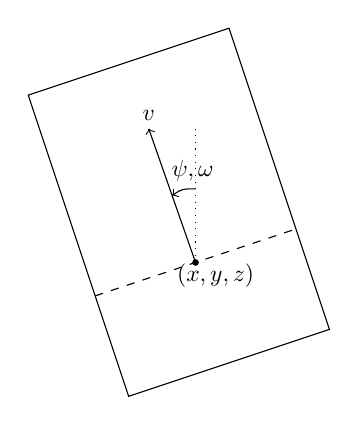
\begin{tikzpicture}[scale=0.85, every node/.style={scale=0.85}]
        % --- Draw rectangle car ---
        \draw (0,0) -- (3,1) -- (1.5,5.5) -- (-1.5,4.5) -- cycle;
        \draw[dashed] (-0.5,1.5) -- (2.5,2.5) node[pos=0.6, anchor=north] {$(x,y,z)$};
        \draw[->] (1,2) node[circle,fill,inner sep=1pt] {} -- (0.3,4) node[anchor=south] {$v$};
        \draw[dotted] (1,2) -- (1,4);
        \draw[<-] (0.65,3) .. controls (0.8,3.1) .. (1,3.1) node[pos=0.5, anchor=south] {\hspace{0.3cm}$\psi, \omega$};
        % ---
    \end{tikzpicture}
    \caption{\label{fig:motionmodel} The notation in the motion model related to the target vehicle.}
\end{figure}

Note that if the host is moving while tracking the target, at each sample, \ie frame, the state of the target must be compensated with respect to the host's ego motion.
It has been omitted from \eqref{eq:motionmodel} in order to simplify the expressions and as mentioned in \Chapterref{cha:intro}, the thesis deals only with host cars with no ego motion.
A generalized formulation of the compensation is
%
\begin{equation}
	\bm{x}_{k+1} = \bm{f}_{\text{Motion}}\left( \bm{f}_{\text{Ego}}(\bm{x}_k) \right),
\end{equation}
%
where $\bm{f}_{\text{Ego}}$ is the function which compensates for the host's ego motion and $\bm{f}_{\text{Motion}}$ is the motion model \eqref{eq:motionmodel}.
%
\begin{table}[!ht]
\centering
\caption{\label{tab:motionmodel} The variables in the motion model for the target.}
    \begin{tabular}{|c|p{9cm}|}
    \hline
    \textbf{Notation} & \textbf{Definition} \\
    \hline
    \rule{0pt}{1.1em}
    $\bm{x}$ & The target's state vector, \ie $\bm{x} = \left(x, y, z, v, \psi, \omega \right)^T$. \\
    \hline
    $x$ & The target's position in the $x$-direction of the host's coordinate system. \\
    \hline
    $y$ & The target's position in the $y$-direction of the host's coordinate system. \\
    \hline
    $z$ & The target's position in the $z$-direction of the host's coordinate system. \\
    \hline
    $v$ & The velocity of the target in the $x$-direction of the target's coordinate system. \\
    \hline
    $\psi$ & The yaw angle of the target compared to the host. \\
    \hline
    $\omega$ & The yaw rate of the target. \\
    \hline
    \end{tabular}
\end{table}

\section{Measurement Vehicle Model}
In order to estimate the orientation and angular rate, \ie the heading of a target, a measurement model must be constructed.
In \Figureref{fig:vehiclemodel}, the target vehicle is modelled as a rectangle.
The notation used in \Figureref{fig:vehiclemodel} is further described in \Tableref{tab:vehiclemodel}.
Since no direct distance measurement can be obtained, two assumptions about the width and length of the target must be used.

\begin{figure}[!ht]
    \centering
    \hspace{2cm}
    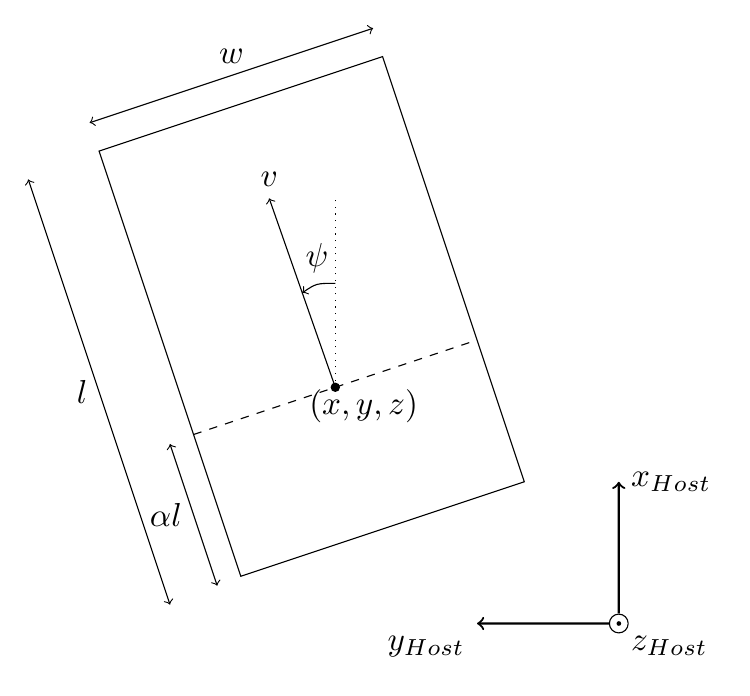
\begin{tikzpicture}[scale=1.2, every node/.style={scale=1.2}]
        % --- Draw rectangle car ---
        \draw (0,0) -- (3,1) -- (1.5,5.5) -- (-1.5,4.5) -- cycle;
        \draw[dashed] (-0.5,1.5) -- (2.5,2.5) node[pos=0.6, anchor=north] {$(x,y,z)$};
        \draw[->] (1,2) node[circle,fill,inner sep=1pt] {} -- (0.3,4) node[anchor=south] {$v$};
        \draw[dotted] (1,2) -- (1,4);
        \draw[<-] (0.65,3) .. controls (0.8,3.1) .. (1,3.1) node[pos=0.5, anchor=south] {$\psi$};
        % ---

        % --- Draw lines for length and width ---
        \draw[<->] (-0.25,-0.1) -- (-0.75,1.4) node[pos=0.5, anchor=east] {$\alpha l$};
        \draw[<->] (-0.75,-0.3) -- (-2.25,4.2) node[pos=0.5, anchor=east] {$l$};
        \draw[<->] (-1.6,4.8) -- (1.4,5.8) node[pos=0.5, anchor=south] {$w$};
        % ---

        % --- Host coordinate system ---
        \node[draw,circle,inner sep=2pt] (hostorigin) at (4,-0.5) {};
        \draw[thick, ->] (hostorigin) node[anchor=north west] {$z_\text{Host}$} -- (4,1) node[anchor=west] {$x_\text{Host}$};
        \draw[thick, ->] (hostorigin) node[circle,fill,inner sep=0.5pt] {} -- (2.5,-0.5) node[anchor=north east] {$y_\text{Host}$};
    \end{tikzpicture}
    \caption{\label{fig:vehiclemodel} The model of a target vehicle. The direction of the $x$-axis of the host's coordinate system coincides with the target's $x$-axis when the yaw angle $\psi$ is zero.}
\end{figure}

\begin{table}[!ht]
\centering
\caption{\label{tab:vehiclemodel} Notations used for describing the target vehicle.}
    \begin{tabular}{|c|p{9cm}|}
    \hline
    \textbf{Notation} & \textbf{Description} \\
    \hline
    $(x,y,z)$ & World coordinates of the target's position in the host's coordinate system. \\
    \hline
    $v$ & The velocity of the target, \ie the target's absolute velocity. \\
    \hline
    $\psi$ & Yaw angle of the target compared to the host. \\
    \hline
    $w$ & Assumed width of the target. \\
    \hline
    $l$ & Assumed length of the target. \\
    \hline
    $\alpha$ & Ratio describing the length of the car behind the rear axis. \\
    \hline
    \end{tabular}
\end{table}

By using the detection methods describes in \Sectionref{sec:objectdetection}, image measurement models can be derived.

\newpage

\subsection{ROI Horizontal Center Position Measurement}

First, we have the measurement of the horizontal center position of the \abbrROI.
In \Figureref{fig:measurementmodelhcp} a geometric view of the measurement is presented.
The observation is the middle of the back, or the front, of the target.
By utilizing the properties of the pinhole camera model, the measurement equation is
%
\begin{equation}
\begin{split}
    p_{\text{HCP, back}} &= -f_u \frac{y + (0,1,0) \rotmat(\psi) (- \alpha l,0,0)^T}{x + (1,0,0) \rotmat(\psi) (- \alpha l,0,0)^T} + e_{\text{HCP, back}}\\
    &= -f_u \frac{y - \alpha l \sin(\psi)}{x - \alpha l \cos(\psi)} + e_{\text{HCP, back}},
\end{split}
\end{equation}
%
where $e_{\text{HCP, back}}$ is the measurement noise and $\rotmat$ is the \spacedim{3} rotation matrix defined as
\begin{equation*}
	\rotmat(\theta) =
	\begin{pmatrix}
		\cos\theta & -\sin\theta & 0 \\
		\sin\theta & \cos\theta & 0 \\
		0 & 0 & 1
	\end{pmatrix}.
\end{equation*}
The measurement is the the number of pixels offset for the horizontal center position, compared to the center of the image in the $u$-direction.
This is illustrated in \Figureref{fig:roihcp}.
If instead the front of the target is observed, the factor $\alpha$ is changed to $\alpha-1$ (the point $((1-\alpha)l,0,0)^T$ is observed instead) and the resulting measurement equation is
%
\begin{equation}
    p_{\text{HCP, front}} = -f_u \frac{y - (\alpha - 1) l \sin(\psi)}{x - (\alpha - 1) l \cos(\psi)} + e_{\text{HCP, front}},
\end{equation}
%
where $e_{\text{HCP, front}}$ is the measurement noise.

% ROI Horizontal Center Position
\begin{figure}[!ht]
    \centering
    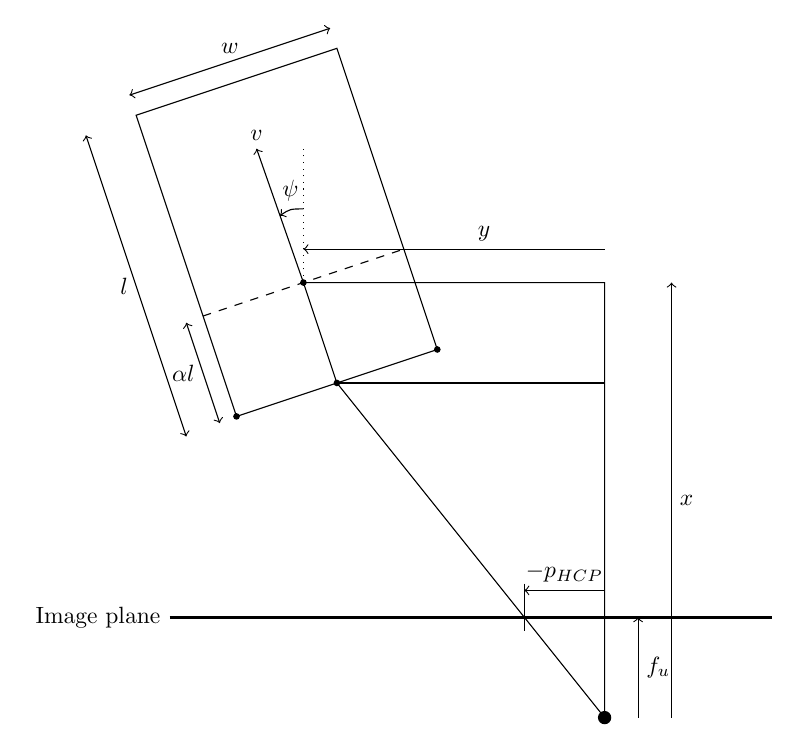
\begin{tikzpicture}[scale=0.85, every node/.style={scale=0.85}]
        % --- Draw rectangle car ---
        \draw (0,0) node[circle,fill,inner sep=1pt] {} -- (3,1) node[circle,fill,inner sep=1pt] {} -- (1.5,5.5) -- (-1.5,4.5) -- cycle;
        \draw[dashed] (-0.5,1.5) -- (2.5,2.5);
        \draw[->] (1,2) node[circle,fill,inner sep=1pt] {} -- (0.3,4) node[anchor=south] {$v$};
        \draw[dotted] (1,2) -- (1,4);
        \draw[<-] (0.65,3) .. controls (0.8,3.1) .. (1,3.1) node[pos=0.5, anchor=south] {$\psi$};
        % ---

        % --- Draw lines for length and width ---
        \draw[<->] (-0.25,-0.1) -- (-0.75,1.4) node[pos=0.5, anchor=east] {$\alpha l$};
        \draw[<->] (-0.75,-0.3) -- (-2.25,4.2) node[pos=0.5, anchor=east] {$l$};
        \draw[<->] (-1.6,4.8) -- (1.4,5.8) node[pos=0.5, anchor=south] {$w$};
        % ---

        % --- Draw image plane and associated lines---
        \coordinate (camOrigo) at (5.5, -4.5);
        \draw[very thick] (-1,-3) node[anchor=east] {Image plane} -- (8,-3);
        \draw[->] (6,-4.5) -- (6,-3) node[pos=0.5, anchor=west] {$f_u$};
        \draw[->] (6.5,-4.5) -- (6.5,2) node[pos=0.5, anchor=west] {$x$};
        \draw[->] (5.5,2.5) -- (1,2.5) node[pos=0.4, anchor=south] {$y$};
        \draw (camOrigo) node[circle,fill,inner sep=2pt] {} -- (5.5,2) -- (1,2) -- (1.5,0.5) node[circle,fill,inner sep=1pt] {} -- cycle;
        \draw (1.5,0.5) -- (5.5,0.5);
        \draw[->] (5.5,-2.6) -- (4.3,-2.6) node[pos=0.5, anchor=south] {$-p_{HCP}$};
        \draw (4.3,-2.5) -- (4.3,-3.2);
        % ---
    \end{tikzpicture}
    \caption{\label{fig:measurementmodelhcp} The measurement model for the \abbrROI horizontal center position when observing the back of the target.}
\end{figure}

\begin{figure}[!ht]
	\centering
	\begin{tikzpicture}
		\node[] at (0,0) {\includegraphics[angle=-90,origin=c,trim={0 0 15cm 0},width=0.85\textwidth]{roi_example}};
		\draw[red, very thick, |->] (0,-0.8) -- (0.7,-0.8) node[anchor=north] {$p_\text{HCP}$};
	\end{tikzpicture}
	\caption{\label{fig:roihcp} The \abbrROI horizontal center position measurement from real-world data.}
\end{figure}

\subsection{ROI Width Measurement}
The width of the \abbrROI is another image measurement model.
It is described in \Figureref{fig:measurementmodelwidth} and \Figureref{fig:roiwidth}.
By taking the difference between $i_1$ and $i_2$, the measurement equation becomes
%
\begin{equation}
\begin{split}
    p_{\text{Width, back}} = &i_1 - i_2 \\
    = &f_u \frac{y + (0,1,0) \rotmat(\psi) (- \alpha l,w/2,0)^T}{x + (1,0,0) \rotmat(\psi) (- \alpha l,w/2,0)^T} \\
    &- f_u \frac{y + (0,1,0) \rotmat(\psi) (- \alpha l,-w/2,0)^T}{x + (1,0,0) \rotmat(\psi) (- \alpha l,-w/2,0)^T} + e_ {\text{Width, back}} \\
    = &f_u \frac{y - \alpha l \sin(\psi) + w \cos(\psi) / 2}{x - \alpha l \cos(\psi) - w \sin(\psi) / 2} \\
    &- f_u \frac{y - \alpha l \sin(\psi) - w \cos(\psi) / 2}{x - \alpha l \cos(\psi) + w \sin(\psi) / 2} + e_ {\text{Width, back}} \\
    = &f_u \frac{(y - \alpha l \sin(\psi) + w \cos(\psi) / 2)(x - \alpha l \cos(\psi) + w \sin(\psi) / 2)}{(x - \alpha l \cos(\psi))^2 - w^2 \sin^2(\psi) / 4} \\
    &- f_u\frac{(y - \alpha l \sin(\psi) - w \cos(\psi) / 2)(x - \alpha l \cos(\psi) - w \sin(\psi) / 2)}{(x -  \alpha l \cos(\psi))^2 - w^2 \sin^2(\psi) / 4} \\
    &+ e_ {\text{Width, back}} \\
    = &-f_u \frac{\alpha l w - y \sin(\psi) w - x \cos(\psi) w}{(x - \alpha l \cos(\psi))^2 - w^2 \sin^2(\psi) / 4} + e_ {\text{Width, back}},
\end{split}
\end{equation}
%
where $e_ {\text{Width, back}}$ is the measurement noise.
If instead the front is observed, the factor $\alpha$ becomes $\alpha - 1$ and the order of the observed points is interchanged yielding the equation
%
\begin{equation}
\begin{split}
    p_{\text{Width, front}} = &i_1 - i_2 \\
    = &f_u \frac{y + (0,1,0) \rotmat(\psi) ((1-\alpha)l,-w/2,0)^T}{x + (1,0,0) \rotmat(\psi) ((1-\alpha)l,-w/2,0)^T} \\
    &- f_u\frac{y + (0,1,0) \rotmat(\psi) ((1-\alpha)l,w/2,0)^T}{x + (1,0,0) \rotmat(\psi) ((1-\alpha)l,w/2,0)^T} + e_ {\text{Width, front}} \\
    = &f_u \frac{(\alpha-1) l w - y \sin(\psi) w - x \cos(\psi) w}{(x - (\alpha-1) l \cos(\psi))^2 - w^2 \sin^2(\psi) / 4} + e_ {\text{Width, front}},
\end{split}
\end{equation}
%
where $e_{\text{Width, front}}$ is the measurement noise.

% ROI Width
\begin{figure}[!ht]
    \centering
    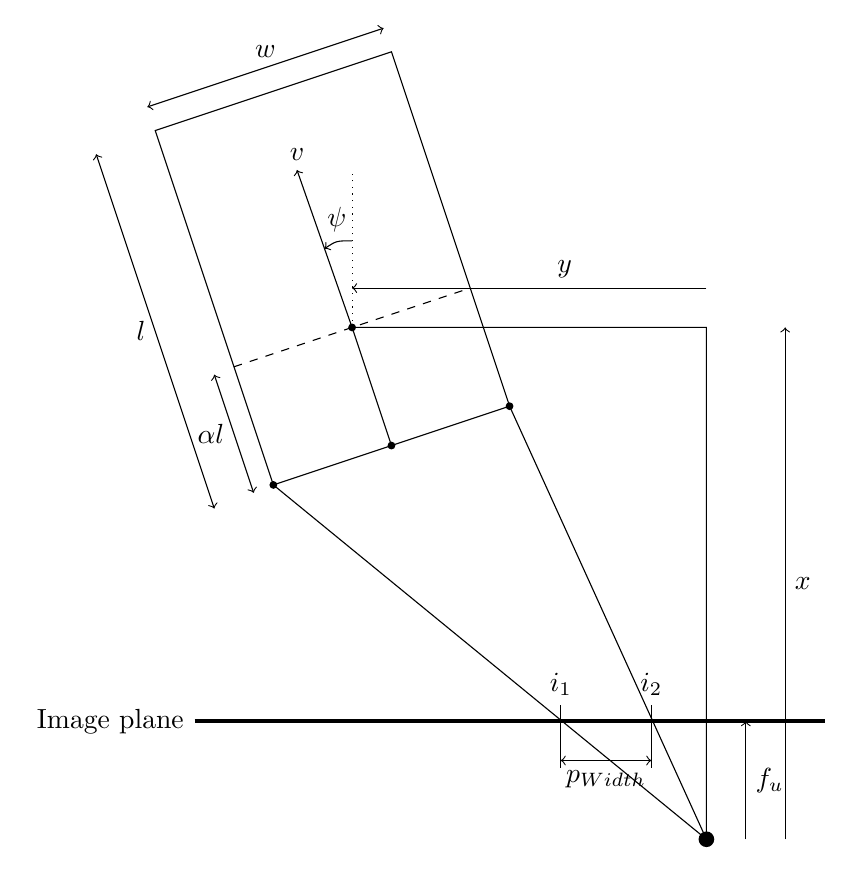
\begin{tikzpicture}
        % --- Draw rectangle car ---
        \draw (0,0) node[circle,fill,inner sep=1pt] {} -- (3,1) node[circle,fill,inner sep=1pt] {} -- (1.5,5.5) -- (-1.5,4.5) -- cycle;
        \draw[dashed] (-0.5,1.5) -- (2.5,2.5);
        \draw[->] (1,2) node[circle,fill,inner sep=1pt] {} -- (0.3,4) node[anchor=south] {$v$};
        \draw[dotted] (1,2) -- (1,4);
        \draw[<-] (0.65,3) .. controls (0.8,3.1) .. (1,3.1) node[pos=0.5, anchor=south] {$\psi$};
        % ---

        % --- Draw lines for length and width ---
        \draw[<->] (-0.25,-0.1) -- (-0.75,1.4) node[pos=0.5, anchor=east] {$\alpha l$};
        \draw[<->] (-0.75,-0.3) -- (-2.25,4.2) node[pos=0.5, anchor=east] {$l$};
        \draw[<->] (-1.6,4.8) -- (1.4,5.8) node[pos=0.5, anchor=south] {$w$};
        % ---

        % --- Draw image plane and associated lines---
        \coordinate (camOrigo) at (5.5, -4.5);
        \draw[very thick] (-1,-3) node[anchor=east] {Image plane} -- (7,-3);
        \draw[->] (6,-4.5) -- (6,-3) node[pos=0.5, anchor=west] {$f_u$};
        \draw[->] (6.5,-4.5) -- (6.5,2) node[pos=0.5, anchor=west] {$x$};
        \draw[->] (5.5,2.5) -- (1,2.5) node[pos=0.4, anchor=south] {$y$};
        \draw (camOrigo) node[circle,fill,inner sep=2pt] {} -- (5.5,2) -- (1,2) -- (1.5,0.5) node[circle,fill,inner sep=1pt] {};
        \draw (camOrigo) -- (0,0) (camOrigo) -- (3,1);
        \draw (3.65,-2.8) node[anchor=south] {$i_1$} -- (3.65,-3.6);
        \draw (4.8,-2.8) node[anchor=south] {$i_2$} -- (4.8,-3.6);
        \draw[<->] (4.8,-3.5) -- (3.65,-3.5) node[pos=0.5, anchor=north] {$p_{Width}$};
        % ---
    \end{tikzpicture}
    \caption{\label{fig:measurementmodelwidth} The measurement model for the \abbrROI width when observing the back of the target.}
\end{figure}

\begin{figure}[!ht]
	\centering
	\begin{tikzpicture}
		\node[] at (0,0) {\includegraphics[angle=-90,origin=c,trim={0 0 15cm 0},width=0.9\textwidth]{roi_example}};
		\draw[red, very thick, <->] (0.2,0.2) -- (1.25,0.2) node[pos = 0.5, anchor=south] {$p_\text{Width}$};
	\end{tikzpicture}
	\caption{\label{fig:roiwidth} The \abbrROI width measurement from real-world data.}
\end{figure}

\newpage

\subsection{ROI Bottom Measurement}

The bottom of the \abbrROI can also be used as a measurement.
The measurement equation, according to \Figureref{fig:measurementmodelbottom}, then becomes
%
\begin{equation}
\begin{split}
    p_{\text{Bottom, back}} &= -f_v \frac{z + (0,0,1) \rotmat(\psi) (- \alpha l,0,0)^T}{x + (1,0,0) \rotmat(\psi) (- \alpha l,0,0)^T} + e_{\text{Bottom, back}} \\
    &= -f_v \frac{z}{x - \alpha l \cos(\psi)} + e_{\text{Bottom, back}},
\end{split}
\end{equation}
%
where $e_{\text{Bottom, back}}$ is the measurement noise.
The measurement is the number of pixels offset for the bottom position, compared the center of the image in the $v$-direction.
This is illustrated in \Figureref{fig:roibottom}.
If instead the front of the target is observed, the factor $\alpha$ is changed to $\alpha-1$ and the measurement equation becomes
%
\begin{equation}
    p_{\text{Bottom, front}} =  -f_v \frac{z}{x - (\alpha - 1) l \cos(\psi)} e_{\text{Bottom, front}},
\end{equation}
where $e_{\text{Bottom, front}}$ is the measurement noise.

% ROI Bottom
\begin{figure}[!ht]
    \centering
    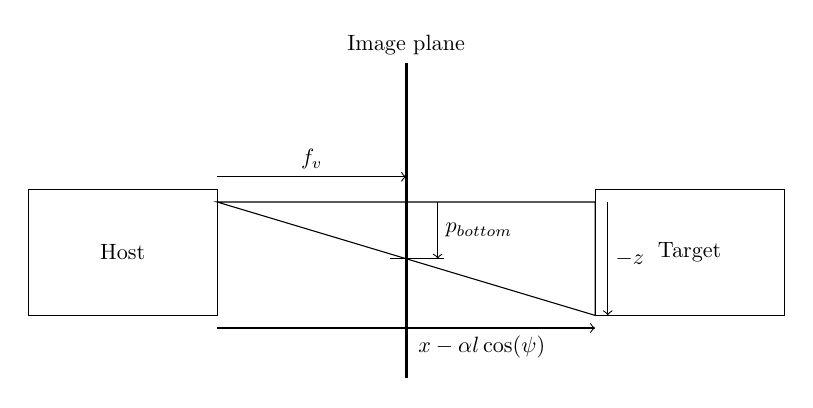
\begin{tikzpicture}[scale=0.8, every node/.style={scale=0.8}]
        % --- Draw image plane ---
        \draw[very thick] (0,3) node[anchor=south] {Image plane} -- (0,-2);
        % ---

        % --- Draw host vehicle and associated lines---
        \draw (-6,-1) rectangle (-3,1) node[pos=0.5] {Host};
        \draw (-3,0.8) -- (3,0.8) -- (3,-1) -- cycle;
        \draw (-0.25,-0.1) -- (0.6,-0.1);
        \draw[->] (0.5,0.8) -- (0.5,-0.1) node[pos=0.5, anchor=west] {$p_{bottom}$};
        \draw[->] (-3,1.2) -- (0,1.2) node[pos=0.5, anchor=south] {$f_v$};
        \draw[->] (-3,-1.2) -- (3,-1.2) node[pos=0.7, anchor=north] {$x - \alpha l \cos(\psi)$};
        % ---

        % --- Draw target vehicle and associated lines ---
        \draw (3,-1) rectangle (6,1) node[pos=0.5] {Target};
        \draw[->] (3.2,0.8) -- (3.2,-1) node[pos=0.5,anchor=west] {$-z$};
        % ---
    \end{tikzpicture}
    \caption{\label{fig:measurementmodelbottom} The measurement model for the \abbrROI bottom point when observing the back of the target.}
\end{figure}

\begin{figure}[!ht]
	\centering
	\begin{tikzpicture}
		\node[] at (0,0) {\includegraphics[angle=-90,origin=c,trim={0 0 15cm 0},width=0.85\textwidth]{roi_example}};
		\draw[red, very thick, |->] (0.65,0) -- (0.65,-0.75) node[pos = 0.5, anchor=west] {$p_\text{Bottom}$};
	\end{tikzpicture}
	\caption{\label{fig:roibottom} The \abbrROI bottom measurement from real-world data.}
\end{figure}

\newpage

\subsection{Angular Rate Measurements}
\label{sec:angratemeas}
By selecting feature points inside the lower half of the \abbrROI, and by using the knowledge of how pairs of feature points have moved between two images, the homography can be estimated.
The lower half of the \abbrROI was selected in order to get feature points lying on a planar surface.
The homography can be decomposed into a rotation matrix $\rotmat$, translation vector $\bm{t}$ and a plane normal vector $\bm{n}$.
Here, the plane normal is the normal of the plane before the homography transformation.
A brief overview of the decomposition will be presented here.
More details can be found in \cite{Malis:2007}.

The homography matrix $\bm{H}$ can be decomposed as
%
\begin{equation}
    \bm{H} = \rotmat + \bm{t} \bm{n}^T.
\end{equation}
%
The rotation matrix $\rotmat$ describes how the estimated plane has rotated between two images.
Since the rotation is relative to the previous image, no absolute angle can be measured.
Instead, the rotation can be used to create the angular rate since the time between two images is assumed to be known, \ie the cameras frame rate.
By extracting the Euler angles from the rotation matrix, the angular rate can be calculated and used as a measurement.
The measurement equation simply becomes
%
\begin{equation}
	y_{\bm{H}} = \omega + e_{\bm{H}},
\end{equation}
%
where $e_{\bm{H}}$ is the measurement noise when using the homography $\bm{H}$ to construct the angular rate measurements.

As mentioned in both \cite{Gabb:2013} and \cite{Malis:2007}, there exist several solutions (up to eight) to the decomposition of the homography matrix.
One problem this method is facing is to decide which solution to choose.
In \cite{Malis:2007}, some methods are described to reduce the number of reasonable solutions from eight to two.
But still, there exists no method to decide the final solution.

Here, some alternatives are proposed on how to select the final solution.
%
\begin{itemize}
    \item Select the solution closest to the current state of the angular rate.

    This will tend to conserve the current state and could fail to detect a sudden change in the angular rate.

    \item Select the solution which has the smallest absolute angular rate.

    Since cars do not usually turns very sharply, one can argue for always choosing the smallest absolute angular rate to be a reasonable alternative.

    \item Use both solutions in the filter and later decide which track to drop.

    Use both measurements and run two parallel hypotheses until one is more likely then the other, and then discard the least likely one.
    This method will however generate an exponential growth of hypotheses.
    This must be taken into consideration if this particular alternative is selected.

    \item Perform empirical studies on synthetic data and see if there is a pattern.

    By using simulated data, the ground truth and the correct decomposition is known and the selected solution can be verified.
\end{itemize}

\subsection{Corner Measurements}
In order to get better information about the heading of the target, using measurements from the corners of the target should improve the estimation.
The available corners for measurements can be seen in \Figureref{fig:measurementmodelcorners} and a hypothetical example from real-world data can be seen in \Figureref{fig:corners}.
The measurement equations can be constructed by writing the \spacedim{3} coordinates of each of the four corners and then project them onto the image plane.
They can be projected in both the image $u$-direction and $v$-direction.

These kinds of measurements in world coordinates can easily be obtained with a stereo camera system, since it has access to depth information from the disparity image.
The purpose of introducing these measurements into the mono camera system, is to show what performance could be expected if these kinds of measurements would be available there as well.
Although, the measurements would be in image coordinates rather then in world coordinates.

The equations of the \spacedim{3} positions of the corners are
%
\begin{align}
	\text{RR}^{\text{\spacedim{3}}} &=
	\left( x,  y, z \right)^T + \rotmat(\psi) \, \left( -\alpha l, \, -w/2, \, 0 \right)^T, \\
	\text{RL}^{\text{\spacedim{3}}} &=
	\left( x,  y, z \right)^T + \rotmat(\psi) \, \left( -\alpha l, \, w/2, \, 0 \right)^T, \\
	\text{FR}^{\text{\spacedim{3}}} &=
	\left( x,  y, z \right)^T + \rotmat(\psi) \; \big( (1-\alpha)l, \, -w/2, \, 0 \big)^T, \\
	\text{FL}^{\text{\spacedim{3}}} &=
	\left( x,  y, z \right)^T + \rotmat(\psi) \; \big( (1-\alpha)l, \, w/2, \, 0 \big)^T.
\end{align}
%
By using the pinhole camera model and projecting the \spacedim{3} positions onto the image plane, the resulting measurement equations for the image $u$-coordinates of the corners are
%
\begin{align}
	p^\text{RR}_u &= -f_u \frac{\text{RR}_y^{\text{\spacedim{3}}}}{\text{RR}_x^{\text{\spacedim{3}}}} + e^\text{RR}_u, \\
	p^\text{RL}_u &= -f_u \frac{\text{RL}_y^{\text{\spacedim{3}}}}{\text{RL}_x^{\text{\spacedim{3}}}} + e^\text{RL}_u, \\
	p^\text{FR}_u &= -f_u \frac{\text{FR}_y^{\text{\spacedim{3}}}}{\text{FR}_x^{\text{\spacedim{3}}}} + e^\text{FR}_u, \\
	p^\text{FL}_u &= -f_u \frac{\text{FL}_y^{\text{\spacedim{3}}}}{\text{FL}_x^{\text{\spacedim{3}}}} + e^\text{FL}_u,
\end{align}
%
where $e^\text{RR}_u, e^\text{RL}_u, e^\text{FR}_u$ and $e^\text{FL}_u$ is the measurement noise, respectively.
The same strategy could also be used to get the $v$-coordinates in the image by interchanging $f_u$ to $f_v$ and $\text{RR}_y^\text{\spacedim{3}}$ to $\text{RR}_z^\text{\spacedim{3}}$ etc.

\begin{figure}[!ht]
    \centering
    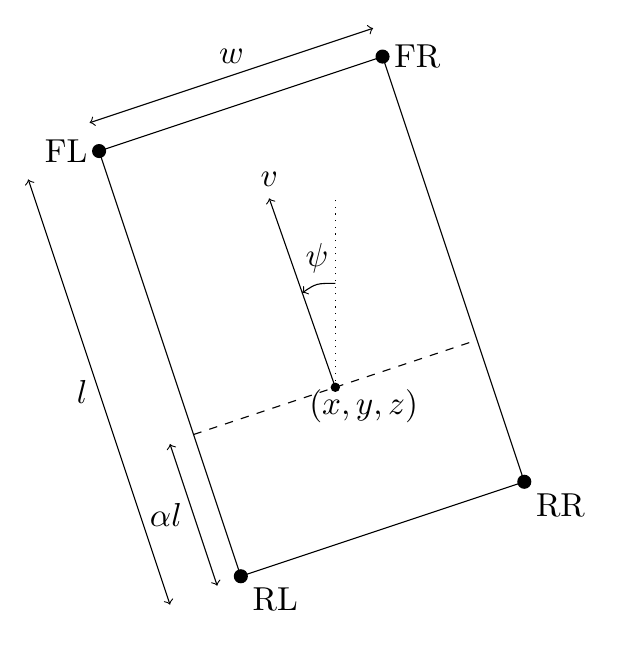
\begin{tikzpicture}[scale=1.2, every node/.style={scale=1.2}]
        % --- Draw rectangle car ---
        \draw (0,0) node[anchor=north west] {RL} node[circle,fill,inner sep=1.5pt] {}  -- (3,1) node[anchor=north west] {RR} node[circle,fill,inner sep=1.5pt] {} -- (1.5,5.5) node[anchor=west] {FR} node[circle,fill,inner sep=1.5pt] {} -- (-1.5,4.5) node[anchor=east] {FL} node[circle,fill,inner sep=1.5pt] {} -- cycle;
        \draw[dashed] (-0.5,1.5) -- (2.5,2.5) node[pos=0.6, anchor=north] {$(x,y,z)$};
        \draw[->] (1,2) node[circle,fill,inner sep=1pt] {} -- (0.3,4) node[anchor=south] {$v$};
        \draw[dotted] (1,2) -- (1,4);
        \draw[<-] (0.65,3) .. controls (0.8,3.1) .. (1,3.1) node[pos=0.5, anchor=south] {$\psi$};
        % ---

        % --- Draw lines for length and width ---
        \draw[<->] (-0.25,-0.1) -- (-0.75,1.4) node[pos=0.5, anchor=east] {$\alpha l$};
        \draw[<->] (-0.75,-0.3) -- (-2.25,4.2) node[pos=0.5, anchor=east] {$l$};
        \draw[<->] (-1.6,4.8) -- (1.4,5.8) node[pos=0.5, anchor=south] {$w$};
        % ---
    \end{tikzpicture}
    \caption{\label{fig:measurementmodelcorners} Measurement model of the corners available to measure on the target.}
\end{figure}

\begin{figure}[!ht]
	\centering
	\begin{tikzpicture}
		\node[] at (0,0) {\includegraphics[angle=-90,origin=c,trim={0 0 16cm 0},width=0.9\textwidth]{corners_example}};
		\node[red,circle,fill,inner sep=1.5pt,label=left:{\color{red}FL}] at (-0.85,-0.65) {};
		\node[red,circle,fill,inner sep=1.5pt,label=below:{\color{red}RL}] at (0.2,-0.85) {};
		\node[red,circle,fill,inner sep=1.5pt,label=right:{\color{red}RR}] at (0.85,-0.75) {};
	\end{tikzpicture}
	\caption{\label{fig:corners} An example of what the measurements from corners could look like.}
\end{figure}

\clearpage

\section{Rotation Estimation with EKF}
Using the motion model and measurement models defined in the preceding sections, the heading can be estimated using the \abbrEKF and by applying \Algorithmref{algo:ekf}.
The state vector is
\begin{equation*}
	\bm{x} =
	\begin{pmatrix}
		x & y & z & v & \psi & \omega
	\end{pmatrix}
	^T
	,
\end{equation*}
and the measurement vector is
\begin{equation*}
	\bm{y} =
	\begin{pmatrix}
		\text{\abbrROI horizontal center position} \\
		\text{\abbrROI bottom} \\
		\text{\abbrROI width} \\
		\text{Angular rate} \\
		\text{Corner coordinates in } u \\
		\text{Corner coordinates in } v
	\end{pmatrix}
	.
\end{equation*}
The process and measurement noise covariance matrices $\bm{Q}$ and $\bm{R}$ are tuning parameters which have to be manually tuned in order to get a good state estimate.

\section{Observability of the Filter}
\label{sec:observabilitymethod}
In order to know if it is possible to get a reasonable solution with the proposed filter structure, the theory from \Sectionref{sec:obsanalysis} is applied.
Since the filter is nonlinear, one can only achieve an observability result around a certain trajectory.
This means that it is not possible to make a general conclusion about the observability of the filter.
Although, by simulating a number of trajectories which could represent interesting real-world scenarios, at least something can be said about the observability.

The Jacobians in each frame in the trajectory have to be calculated and then \eqref{eq:observabilitytheorem} in \Theoremref{th:observability} can be applied to calculate the observability Gramian of the trajectory.
In order to check if the observability Gramian is invertible, the rank of the matrix can be investigated in each sample.

\section{Monte Carlo Simulations}
One way to get knowledge about the expected performance of the filter, is to use the Monte Carlo method, \ie run simulations multiple times and calculate the mean of all observed results (\abbrRMSE).
By first simulating a trajectory and generating measurements accordingly, one can use the generated measurements to estimate the simulated trajectory.
This enables several things:
\begin{itemize}
	\item The simulated trajectory works as ground truth.
	\item All kinds of trajectories can be simulated.
	\item The noise levels of the measurements are controllable.
	\item The expected performance of the filter can be measured.
\end{itemize}
Using the Monte Carlo method, the same trajectory is simulated multiple times with different noise realizations and the mean of the \abbrRMSE's of the estimated trajectories are calculated.
In this thesis, the number of Monte Carlo runs for each trajectory were selected to 1000.
